\documentclass[12pt,a4paper]{article}
\title{Lab4-Lucene1(构建搜索引擎)}
\usepackage{ctex}
\usepackage{amsmath,amscd,amsbsy,amssymb,latexsym,url,bm,amsthm}
\usepackage{epsfig,graphicx,subfigure}
\usepackage{enumitem,balance}
\usepackage{wrapfig}
\usepackage{mathrsfs,euscript}
\usepackage[usenames]{xcolor}
\usepackage{hyperref}
\usepackage[vlined,ruled,commentsnumbered,linesnumbered]{algorithm2e}
\usepackage{float}
\usepackage{geometry}
\usepackage{listings}
\geometry{a4paper,scale=0.8}
\usepackage[T1]{fontenc}
\usepackage[utf8]{inputenc}
\usepackage{amssymb}
% --- Python code template ---
\usepackage[utf8]{inputenc}
% Default fixed font does not support bold face
\DeclareFixedFont{\ttb}{T1}{txtt}{bx}{n}{12} % for bold
\DeclareFixedFont{\ttm}{T1}{txtt}{m}{n}{12}  % for normal

% Custom colors
\usepackage{color}
\definecolor{deepblue}{rgb}{0,0,0.5}
\definecolor{deepred}{rgb}{0.6,0,0}
\definecolor{deepgreen}{rgb}{0,0.5,0}

\usepackage{listings}

% Python style for highlighting
\newcommand\pythonstyle{\lstset{
language=Python,
basicstyle=\ttm,
morekeywords={self},              % Add keywords here
keywordstyle=\ttb\color{deepblue},
emph={MyClass,__init__},          % Custom highlighting
emphstyle=\ttb\color{deepred},    % Custom highlighting style
stringstyle=\color{deepgreen},
frame=tb,                         % Any extra options here
showstringspaces=false
}}
% Python environment
\lstnewenvironment{python}[1][]
{
\pythonstyle
\lstset{#1}
}
{}

% Python for external files
\newcommand\pythonexternal[2][]{{
\pythonstyle
\lstinputlisting[#1]{#2}}}

% Python for inline
\newcommand\pythoninline[1]{{\pythonstyle\lstinline!#1!}}

% --- Python code template ---


\title{Lab4\quad Lucene1(构建搜索引擎)}
\date{2021.10}
\author{孙济宸\quad \quad 学号:520030910016 \quad  \quad 班级:F2003003}
\begin{document}
\maketitle
\section{实验概览}
\begin{enumerate}
	\item 对Lab3中爬虫获取的大量中文网页进行\textbf{索引},修改IndexFiles.py,将每个网页的\textbf{文件名、存储地址、URL、标题和文本内容}索引化;
	\item 运用\textbf{jieba}分词对网页文本\textbf{分词},方便使用WhitespaceAnalyzer索引和查找;
	\item 修改SearchFiles.py实现搜索,显示搜索结果的\textbf{文件名、存储地址、URL、标题和文本内容}。
\end{enumerate}
\section{实验环境}
\begin{itemize}
	\item Docker
	\item \textbf{beautifulsoup (bs4)}
	\item \textbf{pylucene}
	\item \textbf{jieba}
	\item \textbf{paddle}: jieba启用paddle功能依赖库;需运行pip install paddlepaddle
	\item re (正则表达式)
	\item os

\end{itemize}
\newpage

\section{练习题的解决思路}
\subsection{问题1-IndexFiles建立索引}
\subsubsection{对爬虫的修改} \label{addhtml}
由于在建立索引时需要在doc的field中加入网页的URL,方便查询时显示网页链接,但是个人认为,在添加索引时查询index.txt带来额外性能开销,而且.html文件名不能更改,否则查找不到对应的url。
\\因此我的做法是在爬取网页时将网页自己的URL在爬取完将要写入文件前,\textbf{在html文件头上写入网页本身的URL},这样建立索引时读取.html文件时可直接从文件中获取自身的URL。
\begin{python}
SELF_URL_MARKER  = "SELF_URL_TAG:"
f = open(os.path.join(folder, filename), 'w',encoding='utf-8')
f.write("<!- "+SELF_URL_MARKER + page + " -->" + "\n")  
#写html加入含有自身URL的注释
f.write(str(content))
f.close()
\end{python}
\begin{figure}[H]
	%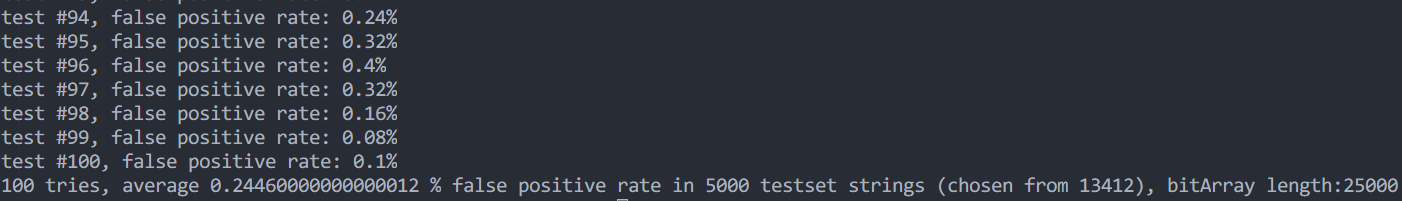
\includegraphics[scale=0.6]{fpr_l.png}
	\centering
	 \caption{含有网页自身URL的自定义注释标签}
\end{figure}
\subsubsection{建立索引}
从目录中读取html文件后,
\begin{itemize}
\item 文件名、文件路径直接从os中获取;
\item title通过BeautifulSoup解析<title><\textbackslash title>标签获取  ( get{\_}self{\_}url(content) )
\item URL通过正则表达式,匹配\ref{addhtml}中添加的自定义注释标签获取。 ( get{\_}title(content) )
\item 文本内容通过clean{\_}html(content)函数去除内嵌代码和html标签后

\end{itemize}
\subsection{问题2-多线程爬虫}
外部IO思路与lab2相同,多线程实现类似BFS,区别是多个线程同时往队列中添加task和获取task。queue中存储的是待爬的url。
先把起始url加入queue,并且设置多个守护线程开始工作。\\
伪代码:\\

\newpage
\section{代码运行结果}
\subsection{问题1(BloomFilter)结果}
m = bitArray长度,n = 测试集大小,k = 哈希函数数量
\subsubsection{m = 5n,k最优}
\begin{figure}[H]
	%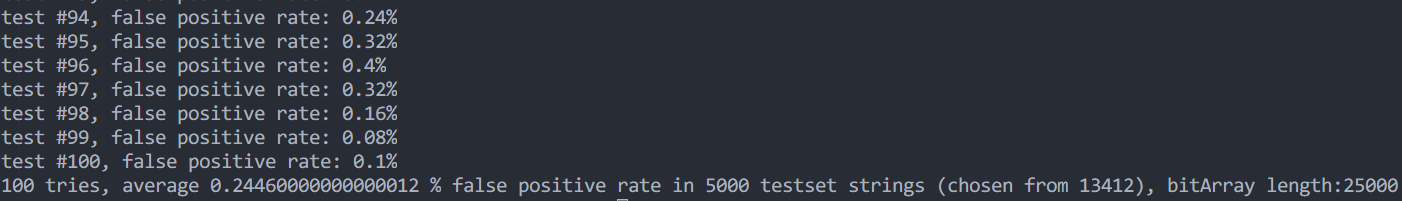
\includegraphics[scale=0.6]{fpr_l.png}
	\centering
	 \caption{FalsePositiveRate- m = 5n}
\end{figure}
\subsubsection{m = 20n,k最优}
\begin{figure}[H]
	%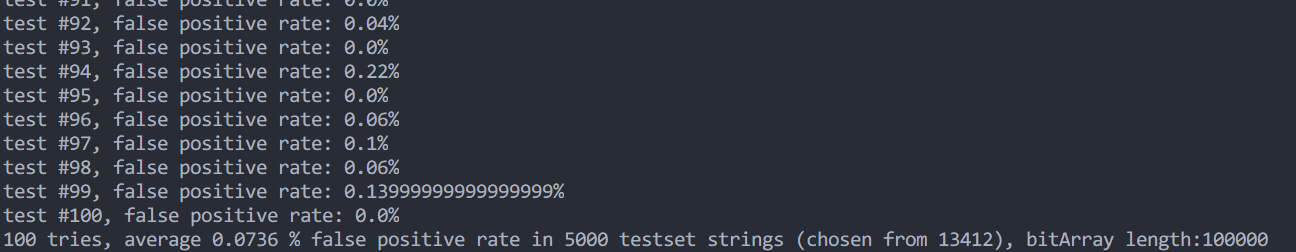
\includegraphics[scale=0.6]{fpr.png}
	\centering
	 \caption{FalsePositiveRate- m = 20n}
\end{figure}

\subsubsection{m = 100n,k最优}
\begin{figure}[H]
	%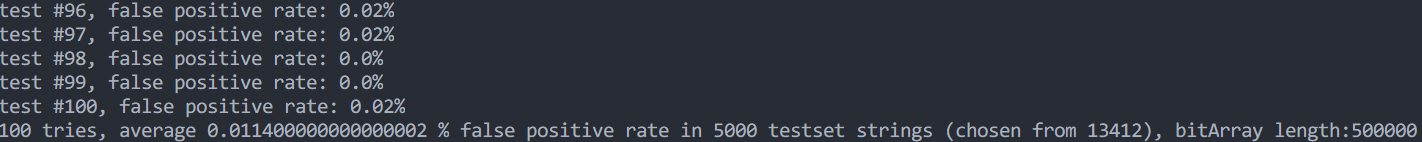
\includegraphics[scale=0.6]{fpr_h.png}
	\centering
	 \caption{FalsePositiveRate- m = 100n}
\end{figure}

可以看到,在k最优的情况下,bitArray长度相比于测试集大小越大,准确率越高(fpr越低),但是牺牲了运行效率。
\subsection{问题2(多线程爬虫)结果}
\begin{figure}[H]
	%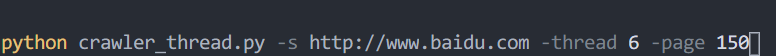
\includegraphics[scale=0.7]{mt0.png}
\end{figure}
\begin{figure}[H]
	 %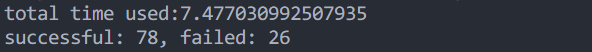
\includegraphics[scale=0.7]{mt1.png}
\end{figure}
\begin{figure}[H]
	 %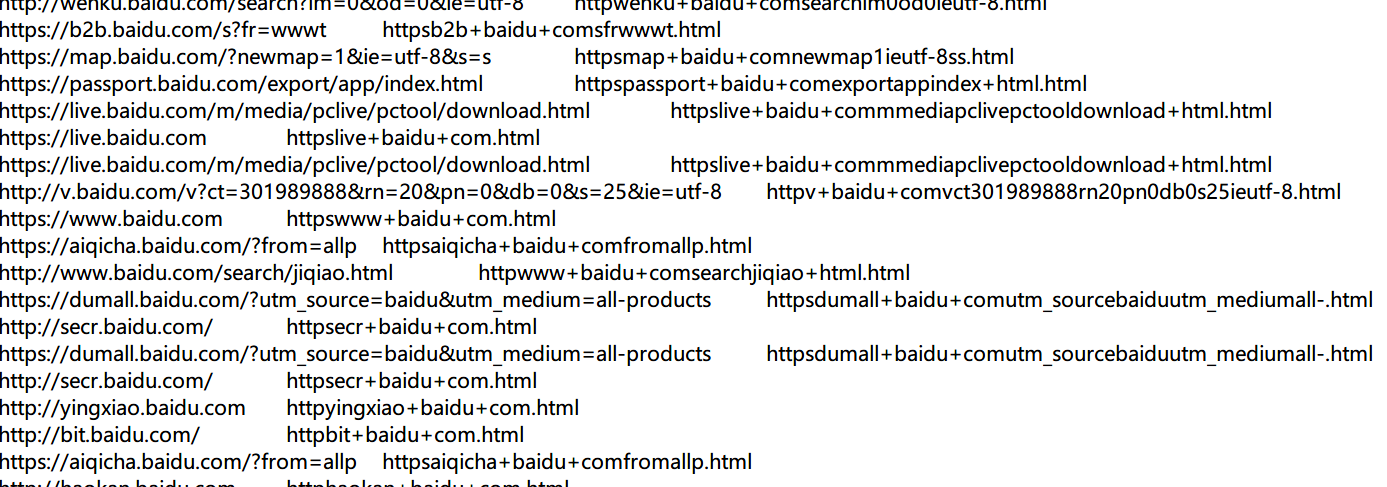
\includegraphics[scale=0.4]{mt2.png}
	 \caption{index.txt}
\end{figure}

完整结果可以运行crawler-thread.py(见readme.txt)


\section{分析与思考}
\begin{itemize}
	\item BloomFilter中使用最优的k时,bitArray长度和准确率正相关,但也会影响运行效率,需要做出权衡。
	\item BloomFilter的hash函数也影响准确率,碰撞少的哈希函数更优
	\item 多线程爬虫为了避免一个线程卡住,很多地方需要加timeout,也要避免加太多锁导致死锁
	\item 在使用线程队列时,要确保task-done无论如何都要调用,否则会出现一个线程卡死队列让队列结束不了
\end{itemize}

\end{document}

